\documentclass{standalone}
\usepackage{tikz}
\usepackage{ctex,siunitx}
\setCJKmainfont{Noto Serif CJK SC}
\usepackage{tkz-euclide}
\usepackage{amsmath}
\usetikzlibrary{patterns, calc,3d}
\usetikzlibrary {decorations.pathmorphing,decorations.pathreplacing,decorations.shapes}
\begin{document}
\small
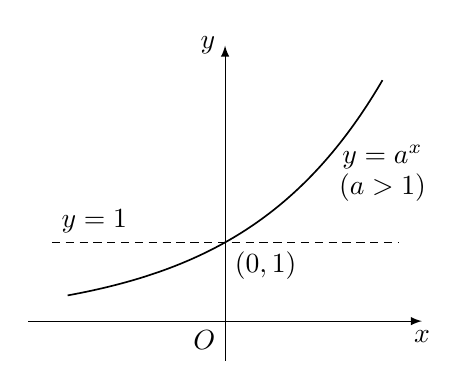
\begin{tikzpicture}[>=latex,scale=1.0]
  \draw[->](-2.5,0)--(2.5,0)node[below]{$x$};
  \draw[->](0,-0.5)--(0,3.5)node[left]{$y$};
  \node at (0,0)[below left]{$O$};
  \draw[densely dashed](-2.2,1)node[above right]{$y=1$}--(2.2,1);
  \draw[semithick,samples=200,domain=-2:2]plot(\x,{pow(1.75,\x)})node[below=20pt]{$y=a^x$};
  \node at (2.0,1.7){$(a>1)$};
  \node at (0,1)[below right]{$(0,1)$};
\end{tikzpicture}
\end{document}